%% ====== Classe du document ============================================
\documentclass[10pt,a4paper]{report}
\usepackage[left=1.5cm,right=1.5cm,top=2cm,bottom=2cm]{geometry}

%% ====== Francisation ==================================================
\usepackage[french]{babel}
\usepackage[T1]{fontenc}
\usepackage[utf8]{inputenc}
\usepackage{textcomp}

%% ====== Personnalisation ============================================
\usepackage{fancyhdr}
	\lhead{}
	\chead{Acquisition et analyse d'image}
	\rhead{M2 IGI 2013-2014}
	\renewcommand{\headrulewidth}{0.3pt}
	\renewcommand{\footrulewidth}{0.3pt}
	\lfoot {hadrien.croubois@ens-lyon.fr}
	\cfoot {- \thepage -}
	\rfoot {}
	\pagestyle{fancy}
\title{Acquisition et analyse d'image}
\author{Hadrien Croubois \and Nicolas Lourdeau}
\date{}

%% ====== Packages pour le texte ========================================
\usepackage{soul}
\usepackage[normalem]{ulem}
\usepackage{fancybox}
\usepackage{moreverb}
\usepackage[table]{xcolor}
%% ====== Packages pour les dessins =====================================
\usepackage{graphicx}
\usepackage{multicol}
\usepackage{multirow}
\usepackage{tikz}
\usepackage{lmodern}
\usepackage{pict2e}

%% ====== Packages pour les maths =======================================
\usepackage{amsmath}
\usepackage{amssymb}
\usepackage{mathrsfs}
\usepackage{bussproofs}
%%\usepackage[ruled,vlined,french]{algorithm2e}
%%\usepackage[squaren,Gray]{SIunits}


%% ====== Reglages generaux =============================================

\usepackage{titlesec}
	\titleformat{\section}[frame]
	{\normalfont}
	{\filright
	\footnotesize
	\enspace Partie \thesection\enspace}
	{6pt}
	{\bfseries\filcenter}
	
	\titleformat{\subsection}[frame]
	{\normalfont}
	{\filright
	\footnotesize
	\enspace \thesubsection\enspace}
	{6pt}
	{\filcenter}
%	{\titlerule
%	\vspace{.8ex}%
%	\normalfont\itshape}
%	{\thesubsection.}{.5em}{}

	\titleformat{\subsubsection}
	{\titlerule
	\vspace{.8ex}%
	\normalfont\itshape}
	{}{.5em}{}

\titleformat{\chapter}[display]
	{\normalfont\bfseries\filcenter}
	{}
	{1ex}
	{\titlerule[2pt]
	\vspace{2ex}%
	\LARGE}
	[\vspace{1ex}%
	{\titlerule[2pt]}]
	
\parindent=10pt

\usepackage{makeidx}
\makeindex
\newcommand\vect{\overrightarrow}

\numberwithin{equation}{subsection}


\graphicspath{{img/}}

\usepackage{subfigure}

%% ======================================================================
\begin{document}
\maketitle
%% ======================================================================
%% ======================================================================

\section*{Philosophie d'utilisation}
Dans le cadre de ce projet, les outils developpés ont toujours été pévu pour etre reutilisés. Ainsi le code se decompose tout naturelllement en deux parties, une librairie facilement compliable au format \texttt{.so} ou \texttt{.dll} fournit avec les fichier en-tête correspondant d'un coté et d'autre part un programme simple permettant d'appeler facillement les fonctionnalitées de la librairie.

Afin de donner differents exemples d'utilisation de la bibliothèque \emph{lenactions}, deux applications sont fournis et donne ainsi differents exemple d'utilisation plus ou moins aux niveaux des fonctionnalités de la bibliotheque.
\begin{itemize}
	\item \textbf{Lenaction} : programme simple, effectuant des appels a la bibliotheque a partir des arguments hard-codé dans le code du programme.
	\item \textbf{LenaSH} : un shell minimaliste interprettant des commandes ecrites dans un langage ad-hoc et proposant ainsi une interface haut niveau pour l'utilisateur.
\end{itemize}

\section*{Outils utlisés}
Afin d'optimiser la portabilité de la bibliothèque, cette derniere ne depend d'aucun autre outil. Ecrite en C/C++ elle gere toutes les etapes du traitement d'images, du chargement de fichier au calcul de contours, en passant par la transition dynamique entre les espaces de couleur \textsc{rgb} et \textsc{hsv}.

Le programme \textbf{LenaSH} utilse les outils flex et bison pour la reconnaissance du langage ad-hoc developpé parallement a la librairie.

Afin de simplifier l'etape de compilation des differents composants du programme sur differentes architectures, nous utilisons l'outil CMake ainsi qu'un script \texttt{./generator}.


\section*{Fonctionnalités}

De nombreux algorithmes sont actuellement deployés dans la bibliotheque a differents niveau:

\begin{itemize}
	\item Pixel :
		\begin{itemize}
			\item Convertion d'espace de couleur
			\item Operateurs de fusion (quadratique, angle)
		\end{itemize}
	\item Image :
		\begin{itemize}
			\item Chargement/Sauvegarde au format \texttt{.ppm} / \texttt{.pgm}
			\item Calcul de seuil
			\item Composition avec un filtre
			\item Assemblage de deux images
			\item seuillage (local, global, histerisis)
			\item affinage de contour
			\item calcul de contour fermés
		\end{itemize}
\end{itemize}

La mise en place de filtre de convolution standart permet par ailleur de calculer simplement les contours via les filtres de Prewitt, Sobel et Kirsch ainsi que d'appliquer un filtre moyenneur gaussien pour lisser l'image.



\section*{Algorithme}
\subsection*{seuillage par histerisis}
Cette operation de seuillage revient a calcul des composantes connexes pour le critere de luminosité $(>low)$ dans l'image. Pour cela on utilise une structure de union find qui garanti un resultat rapide $\mathcal O(n.Ack^{-1}(n))$.

L'ajout d'un drapeau au niveau des composantes connexes permet de marquer les composantes dont un des elements verifie le critere de luminosité $(>high)$.

On ne garde ensuite que les pixels appartenants a une composante connexe marqué.

\subsection*{Affinage de contour}
Pour cette operation, on se base sur une image de contour obtenue a partir de l'operateur de melange \texttt{angle} appliqué a deux gradients.

L'angle decrivant localement le contour (azimut du gradient) est discrétisé et permet de parcourir localement la largeur du contour. En ne gardant que le pixel au centre de ce contour on arrive a garder un contour fidéle, peu bruité et limitant les trous.

\subsection*{Fermeture des contour}
Pour cette operation, nous avons developpé un algorithme a vague proche de ceux utilisés en systeme distribué pour la communication sur des grilles de processeurs.

Ici chaque pixel est une entité pouvant etre dans 4 etats different :
\begin{itemize}
	\item \emph{Vide}
	\item \emph{Champ}
	\item \emph{Contour}
	\item \emph{Ancre}
\end{itemize}

Au debut de l'algorithme, on part d'un contour affiné dont les pixels sont dans l'etat \emph{Contour} tandit que le fond est dans l'etat \emph{Vide}.

La premiere passe se charge de detecter les Ancres parmit des pixels du Contours, pour cela on detecte tout ceux qui ont soit aucun voisin (ancres d'adjacence 2) ainsi que ceux qui sont en bord de contour (soit un unique voisin, soit deux voisin collés) et qui sont des ancres d'adjacence 1.

Les ancres sont les points d'interet qu'il sagit de relié. Leur adjacence correspond au nombre de liaison à former pour faire partie d'un contour fermé.

A partir de la on applique un algorithme de diffusion pour repandre un champ autour des ancres, les pixels passant ainsi de l'etat \emph{Vide} à l'etat \emph{Champ}.

La jonction de champs provoquant la liaison des deux ancres et la diminution de leur adjacence. Si un champ rencontre un pixel d'un contour qui n'est pas dans la composante connexe de l'ancre associé au champ, il s'y accrochera, faisant par la meme occasion diminué l'adjacence de l'ancre dont il provient.
Pour cette diffusion on utilise une file de priorité implementé a partir de tas ainsi qu'une distance basé sur \textsc{BLUE} (best linear unbiased evaluation) et prenant aussi en compte les variations successives du gradient le long du contour a retrouver

Cet algorithme donne de bon de resultats des lors que les la taille des trous est inferieur à la taille des composantes connexes à fermer. 

Voir la section~\ref{resultats}.

\section*{Conclusion}

Apres de longue seances de recherche, nous sommes satisfait de la forme que prend notre bibliotheque. Ne nombreux outils precedements developpé dans le cadre de \texttt{LibImAMXX} (librairie graphique developpé par Hadrien Croubois en M1 et qui a servit de support) sont actuellement en cours d'ajout. Parmit ces outils on compte notament l'affichage des histogrammes avec \texttt{gnuplot}, la normalisation des espaces de couleurs ainsi que le tatouage.

Pour ce qui est des algorithmes developpés, nous sommes relativement content des resultats renvoyés par l'algorithme d'affinage.

L'utilisation de champ dans un algorithme a vague nous semble une piste interressante pour la fermeture des contours. Beaucoup de travail reste cependant a faire, aussi bien pour ce qui est du choix de la fonction de distance que pour les heuristiques de creation des liens d'ancrage.
Nous esperons pouvoir continuer ammeliorer notre algorithme afin de le rendre plus efficace, notament en s'adaptant dynamiquement aux propriété de l'image.



\newpage
\section*{Annexes - Résultats} \label{resultats}


\begin{figure}[ht]
	\center
	\subfigure[Forme geometriques]	{ 
\includegraphics[width=5cm]{imgs/test_image.png} }
	\subfigure[Lena]								{ 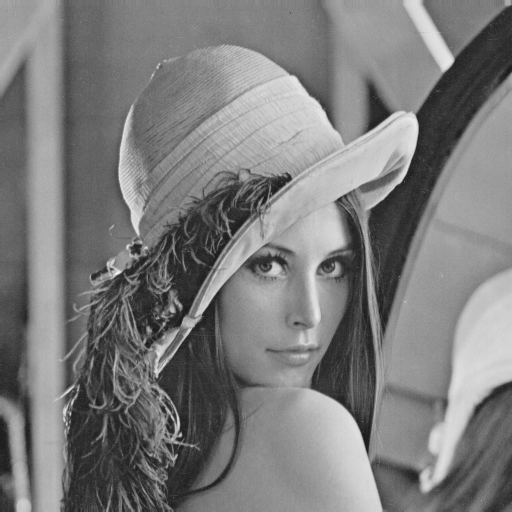
\includegraphics[width=5cm]{imgs/lena512.png} }
	\caption{Images utilisés lors des tests}
\end{figure}

\begin{figure}[ht]
	\center
	\subfigure[Gradient horizontal]	{ 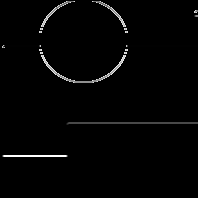
\includegraphics[width=5cm]{imgs/test/1a_hGrad.png} }
	\subfigure[Gradient vertical]		{ 
\includegraphics[width=5cm]{imgs/test/1b_vGrad.png} }
	\subfigure[Gradient composé]		{ 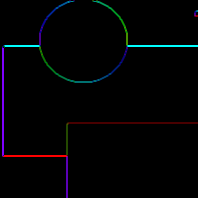
\includegraphics[width=5cm]{imgs/test/2_gTone.png} }
	\subfigure[Contour seuillé]			{ 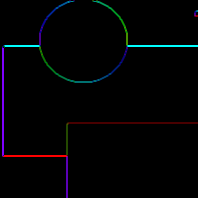
\includegraphics[width=5cm]{imgs/test/3_Border.png} }	
	\subfigure[Contour affiné]			{ 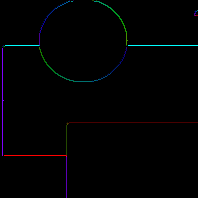
\includegraphics[width=5cm]{imgs/test/4_Affined.png} }
	\subfigure[Contour fermé]				{ 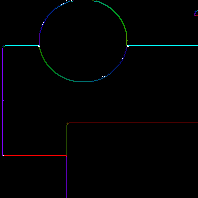
\includegraphics[width=5cm]{imgs/test/5_final.png} }
	\caption{Résultats intermediaire pour des formes simples}
\end{figure}

\begin{figure}[ht]
	\center
	\subfigure[Gradient horizontal]				{ 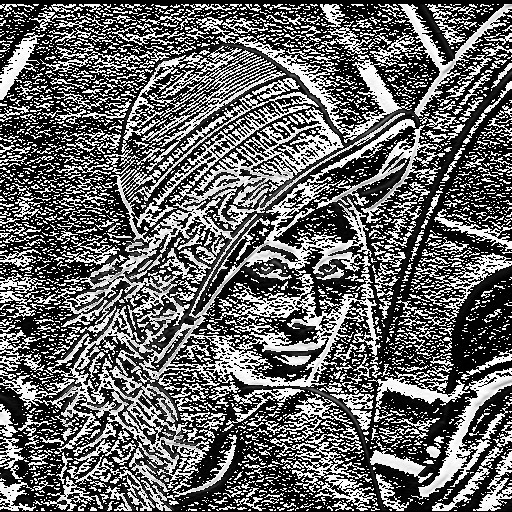
\includegraphics[width=5.5cm]{imgs/lena/1a_hGrad.png} }
	\subfigure[Gradient vertical]					{ 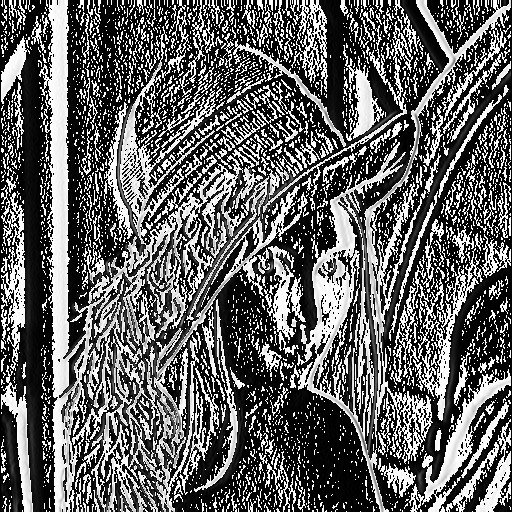
\includegraphics[width=5.5cm]{imgs/lena/1b_vGrad.png} }
	\subfigure[Gradient composé]					{ 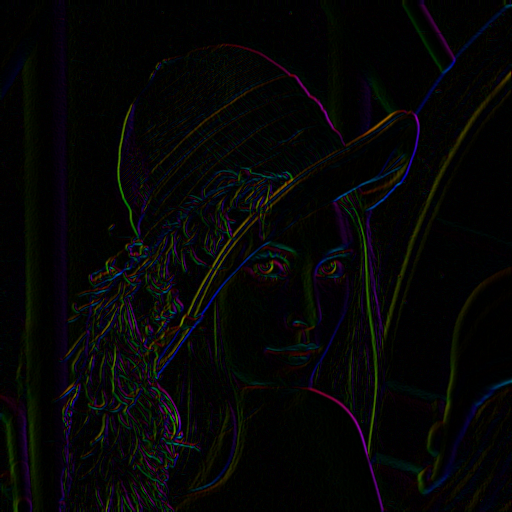
\includegraphics[width=5.5cm]{imgs/lena/2_gTone.png} }
	\subfigure[Contour seuillé]						{ 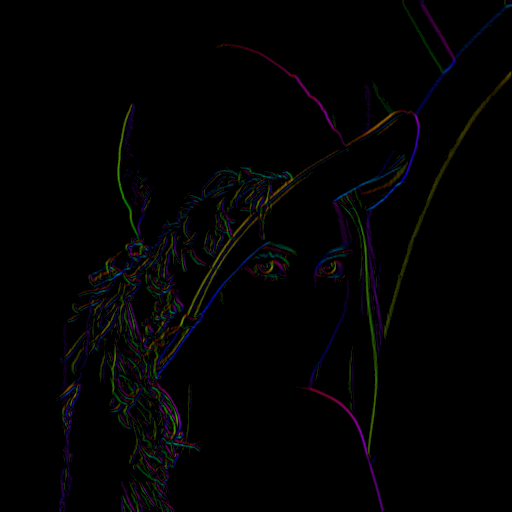
\includegraphics[width=5.5cm]{imgs/lena/3_Border.png} }	
	\subfigure[Contour affiné]						{ 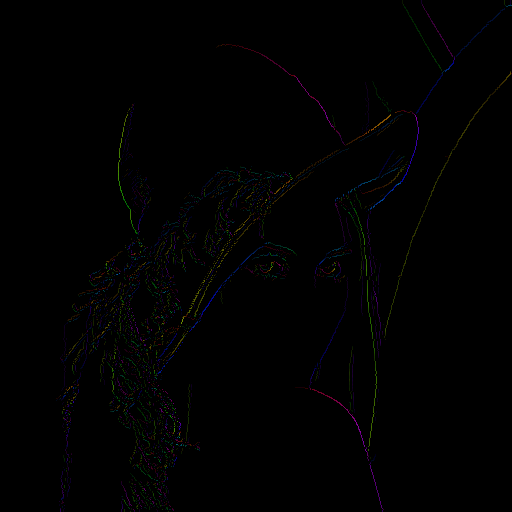
\includegraphics[width=5.5cm]{imgs/lena/4_Affined.png} }
	\subfigure[Points d'ancrage]					{ 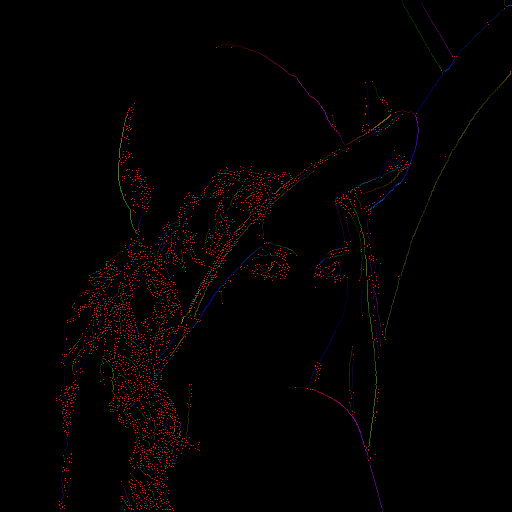
\includegraphics[width=5.5cm]{imgs/lena/5a_final_anchors.png} }
	\subfigure[Limites de la diffusion]		{ 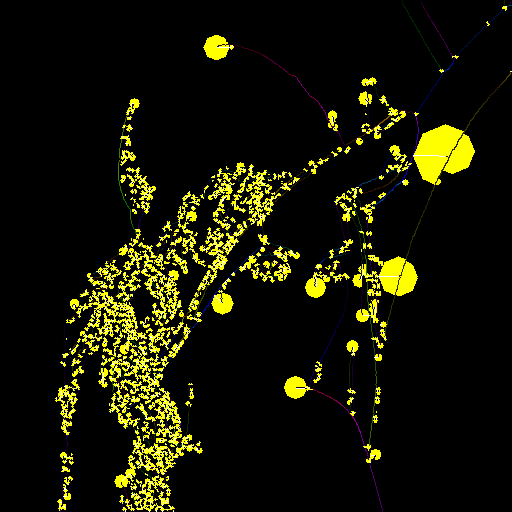
\includegraphics[width=5.5cm]{imgs/lena/5b_final_diffusion.png} }
	\subfigure[Apres fermeture]						{ 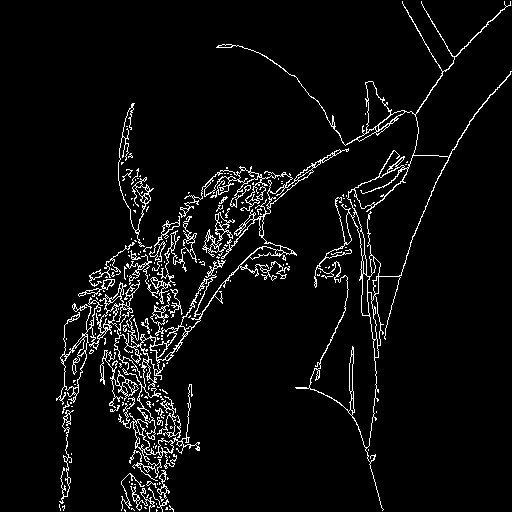
\includegraphics[width=5.5cm]{imgs/lena/5c_final_white.png} }
	\caption{Résultats intermediaire pour Lena}
\end{figure}



\end{document}
